\documentclass{article}
\usepackage{leonine,amsmath,amssymb,amsthm,graphicx}
\setkeys{Gin}{width=\linewidth,totalheight=\textheight,keepaspectratio}
\graphicspath{{graphics/}}
% Prints a trailing space in a smart way.
\usepackage{xspace}
% Inserts a blank page
\newcommand{\blankpage}{\newpage\hbox{}\thispagestyle{empty}\newpage}
% \usepackage{units}
% Typesets the font size, leading, and measure in the form of 10/12x26 pc.
\newcommand{\measure}[3]{#1/#2$\times$\unit[#3]{pc}}

\theoremstyle{definition}
\newtheorem{pred}[thm]{Prediction}

\title{Askesis: Negative Pathway 2} \author{Eric Purdy}

\begin{document}

\maketitle
\section{Overview}

The purpose of the negative pathway is to filter out potential
movements produced by the positive pathway, leaving only the desired
movements as output from the deep nuclear cells. Our theory of the
negative pathway is very similar to the perceptron model of Albus,
although we modify the input to each perceptron slightly.

\section{Purkinje Cells and Basket Cells}
\label{sec-purkinje}

Let $G_i(t)$ be the firing of the $i$-th granular cell at time $t$.

We model the basket cell as 
$$B_j(t) = \sigma \left(\sum_i W^-_{ij} G_i(t) +\theta^-_j \right).$$

We model the Purkinje cell as
$$P_j(t) = \sigma \left(\sum_i W^+_{ij} G_i(t) +\theta^+_j - \alpha B_j(t) \right).$$

We will use a simpler model for the combined basket cell-Purkinje cell
pair:
\begin{align*}
P_j(t) &= \sigma \left(\sum_i (W^+_{ij}-W^-_{ij}) G_i(t) + (\theta^+_j
- \theta^-_j)\right)\\ &= \sigma \left(\sum_i W_{ij} G_i(t) +\theta_j \right),
\end{align*}
where the $W_{ij}$ and $\theta_j$ are free to take on both positive
and negative values.

Let $y_j(t)$ be $1$ if the $j$-th inferior olive cell fires at time
$t$, and $-1$ otherwise. We assume that the inferior olive cells are
in one-to-one correspondence to the Purkinje cells, which is a slight
simplification.

In order to best set the weights $W_{ij}$ and bias $\theta_j$ of the
$j$-th Purkinje cell, we minimize the following function:
$$L(\{W_{ij}\}, \{\theta_j\}) = \sum_t y_j(t) \left(W_{ij} G_i(t) +
\theta_j\right) + \lambda \sum_i W_{ij}^2. $$ 
This rewards us for having the Purkinje cell activation ($W_{ij}
G_i(t) + \theta_j$) low when the climbing fiber is active
($y_j(t)=1$), and for having the Purkinje cell activation high when
the climbing fiber is inactive ($y_j(t)=-1$). Since the Purkinje cell
suppresses the corresponding deep nuclear cell, and the climbing fiber
encodes the information that we want the corresponding deep nuclear
cell to fire, this is the desired behavior.

The term $\lambda \sum_i W_{ij}^2$ is necessary to prevent the weights
from increasing without bound. It favors parameter settings with
smaller weights, which are thought of as being ``simpler'' in the
machine learning literature; favoring smaller weights is thus a form
of Occam's Razor. The constant multiplier $\lambda$ controls the
tradeoff between this term and the other term. The larger $\lambda$
is, the more the algorithm will favor model simplicity (small weights)
over fitting the data well.

This can be compared with the support vector machine (SVM), an
algorithm that minimizes the following function:
$$L(\{W_{ij}\}, \{\theta_j\}) = \sum_t \left[ 1+y(t)\left(\sum_i
  W_{ij} G_i(t) + \theta_j\right)\right]_+ + \lambda \sum_i
W_{ij}^2,$$ where $[a]_+$ is zero if $a$ is negative, and
equal to $a$ otherwise. The difference between the two is that
the SVM uses the ``hinge loss'' while we are simply using a linear
loss function. This difference means that we get extra credit for
being more certain that we are right; with the hinge loss, we are
penalized a lot when we are certain but wrong, but not rewarded for
being more certain when we are right. These loss functions, as well as
the step loss function, are shown in Figure \ref{fig-hinge}; the hinge
loss is a sort of combination of the step loss function and the linear
loss function.

\begin{figure}
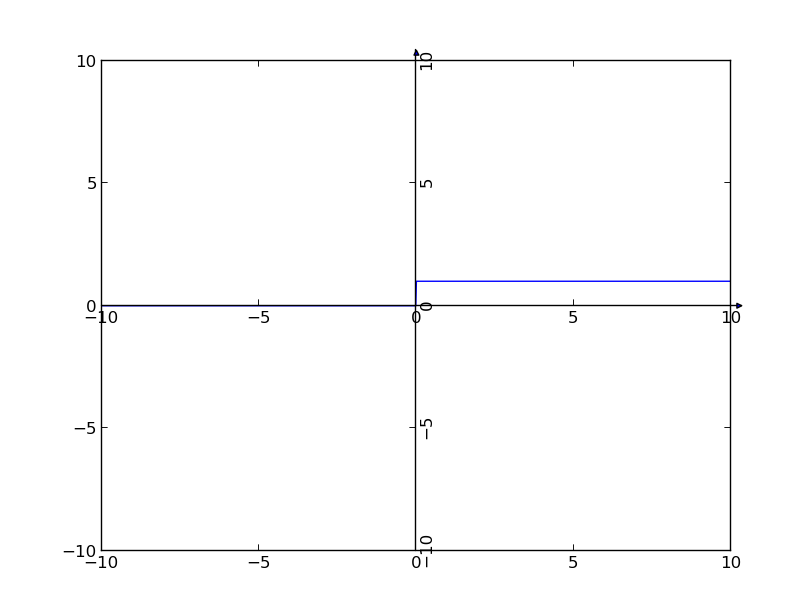
\includegraphics[width=0.3\linewidth]{step_loss.png}
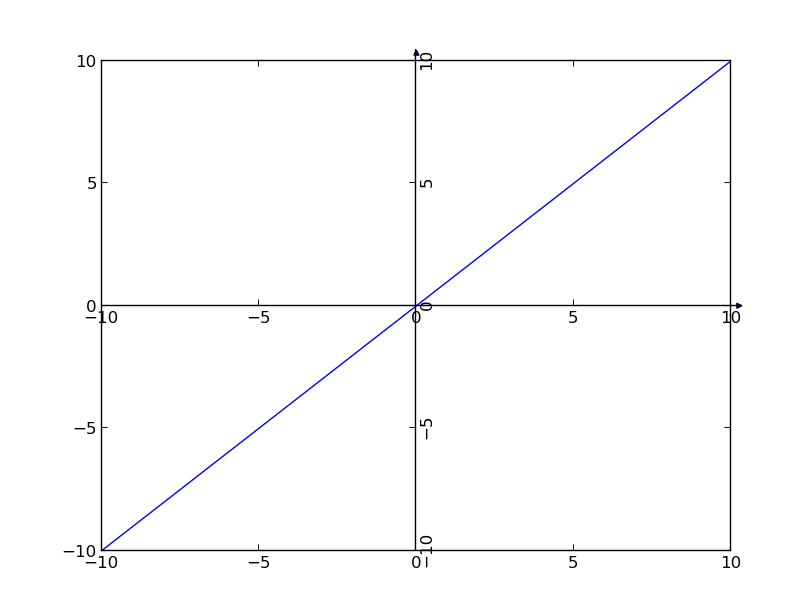
\includegraphics[width=0.3\linewidth]{linear_loss.png}
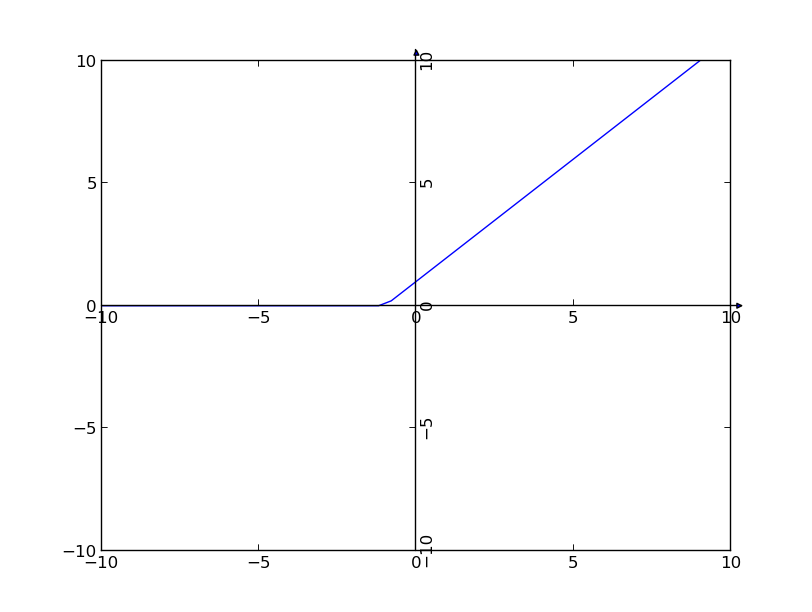
\includegraphics[width=0.3\linewidth]{hinge_loss.png}
\caption{Various loss functions: the step loss function, the linear loss function, and the hinge loss function.}
\label{fig-hinge}
\end{figure}

The partial derivatives are:
\begin{align*}
\frac{\partial L(W)}{\partial W_{ij}} &= \sum_t y(t) G_i(t) + 2\lambda W_{ij}\\
\frac{\partial L(W)}{\partial \theta_j} &= \sum_t y(t).\\
\end{align*}
Using stochastic gradient descent (since we want to minimize
$L(\{W_{ij}\}, \{\theta_j\})$), this leads to the update rules
\begin{align*}
\Delta W_{ij} &= -\eta y_j(t) G_i(t) - \frac{2\eta\lambda}{T} W_{ij}\\
\Delta \theta_j &= -\eta y_j(t). \\
\end{align*}
We apply this to the actual synapse weights and cell biases by adding
$\frac{1}{2}\Delta W_{ij}$ to the weight $W^+_{ij}$ and
$-\frac{1}{2}\Delta W_{ij}$ to the weight $W^-_{ij}$, and adding
$\frac{1}{2}\Delta \theta_j$ to $\theta^+_j$ and adding
$-\frac{1}{2}\Delta \theta_j$ to $\theta^-_j$. This is consistent with
the observed learning behavior at the parallel fiber-Purkinje cell
synapse and the parallel fiber-basket cell synapse:
\begin{itemize} 
\item LTD at the parallel fiber-Purkinje cell synapse when the
  inferior olive cell fires at the same time as the parallel fiber
  ($y_j(t)=1, G_i(t)=1$)
\item LTP at the parallel fiber-Purkinje cell synapse when the
  parallel fiber fires but the inferior olive cell does not
  ($y_j(t)=-1, G_i(t)=1$)
\item LTP at the parallel fiber-basket cell synapse when the inferior
  olive cell fires at the same time as the parallel fiber ($y_j(t)=1,
  G_i(t)=1$)
\item LTD at the parallel fiber-basket cell synapse when the parallel
  fiber fires but the inferior olive cell does not ($y_j(t)=-1,
  G_i(t)=1$)
\item No change when the parallel fiber is inactive ($G_i(t)=0$)
\end{itemize}
We also predict an exponential decay of the weights at both types of
synapse, as well as changes in the intrinsic excitability of the
basket cells and Purkinje cells corresponding to the change in
$\theta^-_j$ and $\theta^+_j$, respectively. The exponential decay
would contribute to memories in the negative pathway being short-lived
relative to memories in the positive pathway, which seems to be the
case.

We have phrased these as if the climbing fiber and parallel fiber
activations should be synchronized, but learning is observed to be
maximized then there is a delay on the order of 100 milliseconds
between the activation of the parallel fiber and the activation of the
climbing fiber. This makes sense: the climbing fiber is activated by
slower, non-cerebellar networks, so its input will always arrive
delayed relative to the relevant stimuli reaching the Purkinje and
basket cells.

\subsection{Symmetry-breaking mechanism for the Purkinje cells}

Each Purkinje cell receives as input, in addition to its input from
the parallel fibers, collaterals from several nearby granular
cells. This input is weighted more highly than that at the parallel
fiber-Purkinje cell synapse. We posit that these collaterals exist to
break the symmetry between Purkinje cells that project to the same
deep nuclear cell, so that we can learn multiple different
classifiers, each of which is capable of suppressing the deep nuclear
cell. Otherwise, adjacent Purkinje cells would receive the same input.
(Recall that nearby inferior olive cells tend to be coupled with gap
junctions, so that the input from the inferior olive would also be the
same for each Purkinje cell.)


\end{document}
